\documentclass[ ]{article}
\usepackage[ ]{graphicx}
\graphicspath{ {./img/} }
\usepackage{indentfirst}
\usepackage[ ]{times}
\title{Descrição dos Elementos Presentes no Sistema}
\date{}
\author{}
\begin{document}
\maketitle
\newpage
\section*{Glossário}
	\begin{enumerate}
		\item Usuário Administrador
		\item Usuário Licitação
		\item Usuário Solicitante
		\item Unidade
		\item Superintendência
		\item Fornecedor
		\item Item
		\item Código NUC
		\item Licitação
		\item Lance
		\item Ata de Registro de Preços
		\item Autorização de Fornecimento e Despacho da AF
		\item Necessidade, Pedidos e Solicitação
	\end{enumerate}
	
\section{Usuário Administrador}
	O usuário Administrador tem todas as permissões do sistema, sua principal função é manter o bom funcionamento da aplicação. Portanto, ele não necessariamente precisa ser vinculado a uma pessoa que pertence a algum dos departamentos aos quais o SIGARP é destinado, mas ele pode fazer modificações e correções que são inerentes a esses setores.

	Por exemplo, caso seja decretado que o modelo de algum documento precise ser modificado, caso esse documento seja gerado automaticamente pelo sistema usando os dados armazenados, o setor competente a esse documento deve solicitar ao usuário administrador para que este faça a alteração do modelo de montagem do documento.
	
	O usuário Administrador poderá também, discricionariamente, alterar, inserir e excluir registros armazenados no sistema que não poderiam ser modificados na aplicação pelos usuários competentes, pois tais modificações não fazem parte de sua natureza.

\section{Usuário Licitação}
	O usuário Licitação tem as permissões que competem ao setor de licitação. Entre elas, poderá fazer o cadastro das licitações, fornecedores, itens e lances. Além de acessar a ferramenta de busca e poder emitir a Ata de Registro de Preços em formato PDF.

\section{Usuário Solicitante}
	O usuário Solicitante geralmente fará parte de uma Unidade Prisional ou algum outro departamento vinculado à Superintendência. Aos usuários pertencentes a esse grupo podem ser atribuídas distintas funções, que representarão sua função na unidade, as mais comum são: Diretor de Unidade, Chefe de Segurança e Coordenador.
	
	O principal uso que este usuário fará deste sistema é o cadastro de Necessidade/Demanda, o qual demonstra à Superintendência e setor de licitação que a unidade está necessitada de tais itens em determinada quantidade para que seja planejada uma nova licitação num futuro próximo.
	
	Outro uso é a solicitação de itens. Após o pregão ter sido concretizado, o usuário solicitante pode pedir para que o setor de licitações adquira uma quantidade dos itens que estão dispostos em ata vigente. Além disso o solicitante pode fazer consultas das licitações para verificar sua situação.

\section{Unidades}
	São, em sua maioria, as unidades prisionais agregadas à Superintendência Regional, mas podem ser também demais setores que se vinculam ao destino das licitações do Setor de Licitação. A própria Superintendência pode ser considerada uma unidade, considerando que um usuário solicitante desta pode cadastrar uma necessidade no sistema.
%	\begin{figure}
		\makebox[\linewidth]{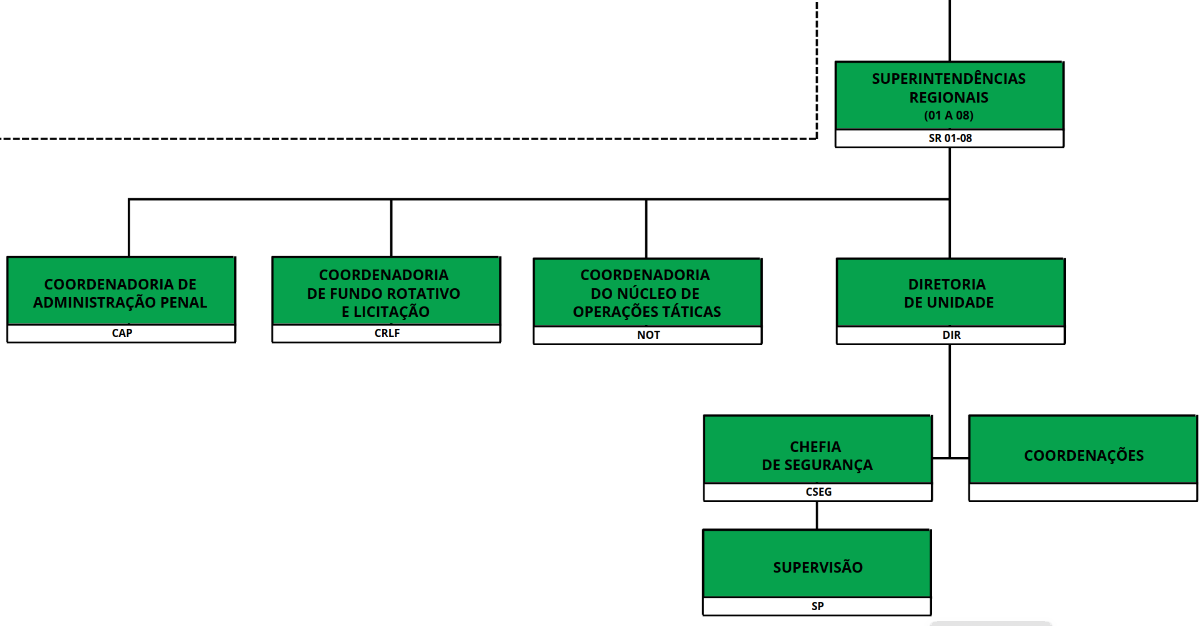
\includegraphics[scale=0.56]{organograma-sejuri.png}}
%		\caption{Organograma Superintendência}	
%	\end{figure}

\section{Fornecedor}
		

\end{document}